\documentclass{article}

\usepackage{url}
\usepackage{graphicx}
\usepackage[abs]{overpic}
\usepackage{pict2e}

\usepackage{xspace}
\usepackage{amsthm}
%\usepackage{alltt,theorem}
\usepackage{algorithm}
\usepackage{algpseudocode}
\algtext*{EndWhile}
\algtext*{EndIf}

\newcommand{\MCCC}{\textsc{MCCC}\xspace}

%\usepackage[linesnumbered]{algorithm2e}
\newcommand{\F}{\mathcal{F}}
\newcommand{\G}{\mathcal{G}}
\newcommand{\f}{\mathcal{f}}

\newcommand{\true}{\textit{true}\xspace}

\makeatletter
\algnewcommand{\LineComment}[1]{\Statex \hskip\ALG@thistlm $//$ #1}
\makeatother

\newtheorem{theorem}{Theorem}
\newtheorem{definition}{Definition}
\newtheorem{proposition}{Proposition}

\begin{document}

\title{Optimal ATPG}
\author{Jessica Davies and Sharad Malik}
\maketitle

\section{Introduction}

When manufacturing digital circuits, it is important to check that the fabricated chip works properly. Chips that are detected to be faulty should be thrown away. It is important that no faulty chips are missed. However, this may be challenging since some faults can be difficult to detect. Furthermore, there are limits to the time and resources that can be invested to test each chip.\\

In order to test whether a given chip is faulty, the standard practise is to run the chip on a set of pre-determined inputs, called test patterns. If any of the test patterns cause the chip to produce output that is contrary to its design, then the chip can be classified as faulty and immediately thrown away.  \\ 

For a given circuit design, and a set of possible faults to be detected, selecting a set of test patterns is called the Automatic Test Pattern Generation (ATPG) problem.\\

In this work, we assume that the circuit is combinational. We focus on detecting chips that are faulty due to exactly one of their lines behaving as if it were stuck at a value (0 or 1). This is commonly known as the stuck-at fault model. Let $\F$ be the set of all stuck-at-0 and stuck-at-1 faults for a circuit $\Phi$.\\

We are interested in finding a set of test patterns, $S$, such that for each stuck-at fault $f \in \F$, there exists a test pattern in $S$ that detects $f$. Such a set of test patterns detects all stuck-at faults, and is said to have complete coverage.\\

\begin{definition}
A set of test patterns $S$ has \textbf{complete coverage} of a set of faults $\F$ if for every fault $f \in \F$, there exists a test pattern $s \in S$ such that $s$ detects $f$.
\end{definition}

Furthermore, we are interested in minimizing the number of test patterns, since this reduces the time required to test each chip. The size of a test set is also known as its compactness. We aim to find a test set that has complete coverage, and such that no other test set with complete coverage is more compact. 

\begin{definition}
A maximally compact, complete-coverage test set, or \textbf{\MCCC}, is a set of test patterns $S_{min}$ that has complete coverage, and such that for any other set $S'$ with complete coverage, $|S'| \geq |S_{min}|$. 
\end{definition}

In the following section, we propose a new approach for calculating a \MCCC test set. 

\section{\MCCC Generation}
\label{sec:alg}

We propose a new algorithm to find an MCCC test set for a given circuit $\Phi$ and set of faults $\F$. The algorithm is shown in Algorithm~\ref{algo:atpg1}.

\begin{algorithm}
\caption{Find an MCCC test set for faults $\F$ of circuit $\Phi$}
\label{algo:atpg1}
\begin{algorithmic}[1]
  \Procedure{\MCCC}{$\Phi, \F$}
  \State $G = $ choose one fault $f \in \F$
  \State $S = \emptyset$
  \State $m = 1$
  \While{true}
    \State $S$ = \textbf{testSet}($\Phi$, $G$, $m$) \Comment{\parbox[t]{.5\linewidth}{Returns a set of $m$ test patterns that detects all faults in $G$, or $\emptyset$ if none exists.}}

    \If{$S == \emptyset$}
        \State $m = m + 1$
        \State $S$ = \textbf{testSet}($\Phi$, $G$, $m$) 
    \EndIf 
    \State $f$ = \textbf{undetected}($\Phi$, $\F\setminus G$, $S$) \Comment{\parbox[t]{.3\linewidth}{$f$ is a fault in $\F$ that is not detected by $S$.}}
    \If{$f$ == null}
        \State \textbf{break} \Comment{$S$ detects all faults in $\F$}
    \Else
        \State $G$ = $G \bigcup \{f\}$
    \EndIf 
    \EndWhile
    \State \textbf{return} $S$
    \EndProcedure
\end{algorithmic}
\end{algorithm}

\begin{theorem}
Algorithm~\ref{algo:atpg1} terminates and returns an \MCCC test set.
\end{theorem}
\noindent \textbf{Proof} At each iteration, either the set of faults $G$ is augmented with a new fault not already in $G$ (lines 10 and 14), or, the loop terminates (line 12). Since the set of all possible faults $\F$ is finite, $G$ can not be augmented an infinite number of times. Therefore the loop, and thus the algorithm, terminates.  When the algorithm terminates, line 12 must have been executed because this is the only way for the loop to terminate. At this time, the current set of test patterns, $S$, detects all faults in $\F$ (by the definition of \textbf{undetected}). Therefore, the algorithm always returns a test set $S$ with complete coverage. It remains to show that the returned test set is of minimum size.  We prove this by induction on the number of loop iterations $k$, by proving that at line 10, there is no test set of size strictly smaller than $m$ that detects all faults in $G$. In the first iteration of the loop, $G$ contains only $1$ fault, and therefore on line 6, $S$ will contain exactly $1$ test pattern. Since $S$ is non-empty on line 7, the condition on line 7 fails and lines 8 and 9 will not be executed. Thus during the first iteration, on line 10 $S$ is a min-size test set that covers the faults in $G$. Let $k \geq 1$ and assume that during loop iteration $k$, on line 10 $S$ is a min-size test set that covers the faults in $G$. We prove that this is also the case for the $k+1^{st}$ iteration. First, on the $k+1^{st}$ iteration of the loop, $G^{k+1}$ will be $G^k \bigcup \{f\}$. If the condition on line 7 fails, then $|S^{k+1}| = |S^k|$, so by the induction hypothesis, $S^{k+1}$ is of minimum possible size to cover $G^k$, and therefore also to cover $G^{k+1}$. Otherwise, if the condition on line 7 succeeds, it means that there is no test set of size $|S^k|$ that detects all faults in $G^{k+1}$. Therefore, any test set that detects all faults in $G^{k+1}$ must have size at least $|S^k|+1$. However, this is the size of the test set returned on line 9 (\textbf{testSet} will not return $\emptyset$ because there \textit{does} exist a test set of size $|S^k|+1$ that detects all faults in $G^{k+1}$: just add a test pattern for the newest fault). So on line 10, in either case, $S^{k+1}$ will be a min-size test set that detects all faults in $G^{k+1}$.         

\section{SAT-based ATPG}

The algorithm proposed in Section~\ref{sec:alg} does not specify how the functions \textbf{testSet} and \textbf{undetected} are implemented. In this section, we describe a possible implementation of these two functions, based on the well-known SAT-based techniques for ATPG.\\  

\subsection{SAT-based Implementation of \textbf{testSet}}
\label{sec:testsetimpl}

Here, we assume that the circuit is irredundant, so that all faults are detectable. We discuss the case where the circuit has undetectable faults in Section~\ref{sec:undetectedimpl} below.  

Figure~\ref{fig:circuit} shows the circuit that we use to implement the \textbf{testSet} function.  This circuit is translated to a CNF formula, and given to a SAT solver. If the formula is satisfiable, the truth assignment returned by the SAT solver will specify $m$ test patterns that detect all faults in $G$. Otherwise, if the SAT solver returns UNSAT, it means there is no set of just $m$ test patterns that can detect all faults in $G$.\\
 
The circuit in Figure~\ref{fig:circuit} mentions sub-circuits $C^f_i$, for each fault $i$ in $G$. These sub-circuits ensure that fault $i$ is detected,  using a standard (or improved) encoding of the test generation problem to SAT~\cite{Larrabee92testpattern,HuanChen_12_2013}. A simple implementation of $C^f_i$ is shown in Figure~\ref{fig:subcircuit}, but in practise, we use the improved encoding of Chen and Marques Silva~\cite{HuanChen_12_2013}.\\

The size of the formula resulting from a CNF encoding of the circuit in Figure~\ref{fig:circuit}, is $O(k(n+m))$ where $n$ is the size of the original circuit $\Phi$, $k$ is the current number of faults $|G|$, and $m$ is the number of test patterns. During the execution of Algorithm~\ref{algo:atpg1}, $k$ begins at $1$, and then grows by exactly $1$ after each iteration of the loop (line 14). Note that $m \leq k$. We hope that the total number of loop iterations will be much less than $|F| = O(n)$. In this case, the largest formula passed to the SAT solver will be significantly smaller than $O(n^2)$.  \\

 
\subsection{SAT-based Implementation of \textbf{undetected}}
\label{sec:undetectedimpl}

Next, we describe the implementation of the second function of Algorithm~\ref{algo:atpg1}, \textbf{undetected}. This function must find a fault in $\F\setminus G$ that is undetected by the current set of test patterns $S$. The general approach we propose is as follows. 


%For each fault $i$ in $\F\setminus G$, and each test pattern $p_j \in S$, we determine whether $p_j$ detects fault $i$ by simulating $p_j$ as input to the original circuit $\Phi$ and the faulty circuit $\Phi^f_i$.  Each simulation can be performed by two calls to a SAT solver, on $p_j \wedge \Phi$, and on $p_j \wedge \Phi^f_i$. Both of these formulas will be satisfiable\footnote{Note that the SAT solver will be able to determine the satisfiability of each formula using unit propagation alone, in linear time. }. The satisfying truth assignments can be compared to determine whether the value of the output variables differs. If so, the pattern $p_j$ detects fault $i$. Otherwise, we try the next test pattern in $S$, until either we find one that detects fault $i$, or we run out of test patterns. If we run out of test patterns to try, then we have found an undetected fault and the simulation of faults is terminated. Therefore, the worst-case running time of \textbf{undetected} is $O(|\F\setminus G| \times |S| \times n)$.  \\

We choose a fault $i \in \F \setminus G$ at random, and check whether it is detected by the current test pattern set $S$. We can check whether fault $i$ is detected by test set $S$ by building a CNF formula like that in Figure~\ref{fig:circuit}, except with only a single sub-circuit $C^f_i$ for the fault $i$, and a single multiplexer whose inputs are fixed to $S$. If the SAT solver returns a solution, then fault $i$ is detected and we must choose another fault at random and try again. If all faults have been determined to be detected by $S$, then we return $\emptyset$ to indicate that $S$ has complete coverage. Otherwise, we return the first fault we find that isn't detected by $S$.     

If the circuit is not irredundant, then before a fault $f$ is returned by \textbf{undetected}, we must first check whether $f$ is detectable. This can be done by calling \textbf{testSet}$(\Phi, \{f\},1)$. If no test pattern is returned, the simulation must continue until an undetected, yet detectable, fault is found.  


%\subsection{Heuristics}
%
%The implementation of \textbf{undetected} can be improved by employing various heuristics, as well as by saving information.  
%
%\subsubsection{Test Pattern Cache}
%\label{sec:testpatterncache}
%Every time a particular test pattern $p_j$ is simulated with fault $i$, we can cache the result of this simulation (i.e., whether $p_j$ detects fault $i$ or not). Then in subsequent iterations, if $p_j$ and fault $i$ are to be simulated again, we can check the cache rather than calling the SAT solver. Since the set of test patterns $S$ changes in every iteration of the loop of Algorithm~\ref{algo:atpg1}, the number of test patterns in the cache may grow to $O(2^\rho \times |\F|)$, where $\rho$ is the number of inputs of $\Phi$. Therefore, it may be necessary to purge part of the cache periodically.\\
%
%\subsubsection{Fault Ordering}
%\label{sec:ordering}
%It is desirable for an undetected fault to be found as quickly as possible during each call to \textbf{undetected}. The \textit{order} in which faults are considered affects the number of faults that must be considered before finding one that is undetected. Intuitively, it is better to consider faults that are unlikely to be detected by $S$ first.  One possible heuristic to order faults is by the number of test patterns that have already been observed to detect the fault. This information is available in the test pattern cache described in Section~\ref{sec:testpatterncache}. We propose to test the faults in increasing order of this metric.\\
%
%\subsubsection{Fault Partitioning}
%The simulation of faults can be parallelized, by partitioning all faults in $\F$ over $\kappa$ separate slave machines: $\F_1,...,\F_\kappa$. When \textbf{undetected} is called, the current test pattern set $S$, and the set of indices of the detected faults $G$, can be communicated to each of the machines. Each machine $j$ will iterate through the faults in $\F_j \setminus G$, and simulate the test patterns in $S$ in order to find an undetected fault if one exists in this partition. If an undetected fault is found by machine $j$, it is sent back to the master machine. This fault can be used immediately to continue the loop iterations of Algorithm~\ref{algo:atpg1}.\\
%
%If the faults are distributed over separate machines, it is no longer possible to maintain a centralized test pattern cache, because it would require a considerable amount of communication from the slave machines to the master. Luckily, the same benefit can be realized by maintaining a separate cache on each slave machine. Since each slave sees the entire set of test patterns $S$, it will have complete information about which patterns detect which faults in its partition, and thus the number of calls to the SAT solver will be reduced by the same amount as if the faults had not been distributed. The fault ordering heuristic proposed in Section~\ref{sec:ordering} can also be implemented on each slave machine by referring to the local cache.\\
%
%There is a trade-off between simulating all test patterns on all faults, so that the cache contains the most complete information possible, and terminating the simulation as soon as an undetected fault is found. If the faults are partitioned over slave machines, then it is possible for the slave machines to continue the simulations even after an undetected fault has been found and returned to the master machine. This is because the master machine is expected to be busy for a considerable amount of time, finding the next set $S$. This is an additional potential benefit to the fault partitioning scheme.
%
%\subsection{Optimized Test Sets}
%The implementation of \textbf{testSet} described in Section~\ref{sec:testsetimpl} uses a SAT solver to find a test set of size $m$ if one exists. However, the test set returned by the SAT solver is \textit{arbitrary}, and we expect that in fact, some test sets are more desirable than others. For example, for sufficiently large $m$ there exists at least one test set that detects \textit{all} faults in $\F \setminus G$. If such a test set is found, then the loop terminates immediately, while otherwise, additional iterations will be required. This suggests that we are interested in finding a test set $S$ that detects all faults in $G$, and the largest number of additional faults in $\F \setminus G$. We propose a heuristic that should help to find such a test set. \\
%
%We propose to add an optimization criteria to the SAT problem described in Figure~\ref{fig:circuit}, so that it becomes a Max-SAT problem. Let $C$ be the CNF formula obtained from Figure~\ref{fig:circuit}. For every Boolean variable $p_{i,j}$ of test pattern $p_i$, we introduce two Boolean variables $b^+_{i,j}$ and $b^-_{i,j}$ which represent setting $p_{i,j}$ to True and False respectively. Every occurrence of the literal $p_{i,j}$ in $C$ is replaced by $b^+_{i,j}$, and every occurrence of the literal $\neg p_{i,j}$ is replaced by $b^-_{i,j}$, to produce a new CNF formula denoted $C^b$. The hard clauses of the Max-SAT instance will be $C^b$, together with clauses $(\neg b^+_{i,j} \vee \neg b^-_{i,j})$ for each $i,j$. These extra clauses assert that both members of a pair $b^+_{i,j}, b^-_{i,j}$ can not be True at the same time. The soft clauses of the Max-SAT instance are $(\neg b^+_{i,j}), (\neg b^-_{i,j})$ for each $i,j$. The soft clauses are used to penalize setting the $b^+$ or $b^-$ variables to True.\\
%
%A solution to the Max-SAT instance will describe a set of $m$ \textit{partial} test patterns. Each partial test pattern specifies values for only a \textit{subset} of the input variables of $\Phi$. However, the partial test patterns still detect all faults in $G$. That is, the values of the partial test pattern variables are sufficient to guarantee that the values of the output variables of $\Phi$ and $\Phi^f_i$ are different, for each fault $i$.\\
%
%How to use the partial test patterns? Maybe it only makes sense to do this optimization after the loop terminates, so that the test patterns have as many unspecified values as possible, which is desirable when setting up finite state controllers to test the chips.



\begin{figure}[t]
\centering
%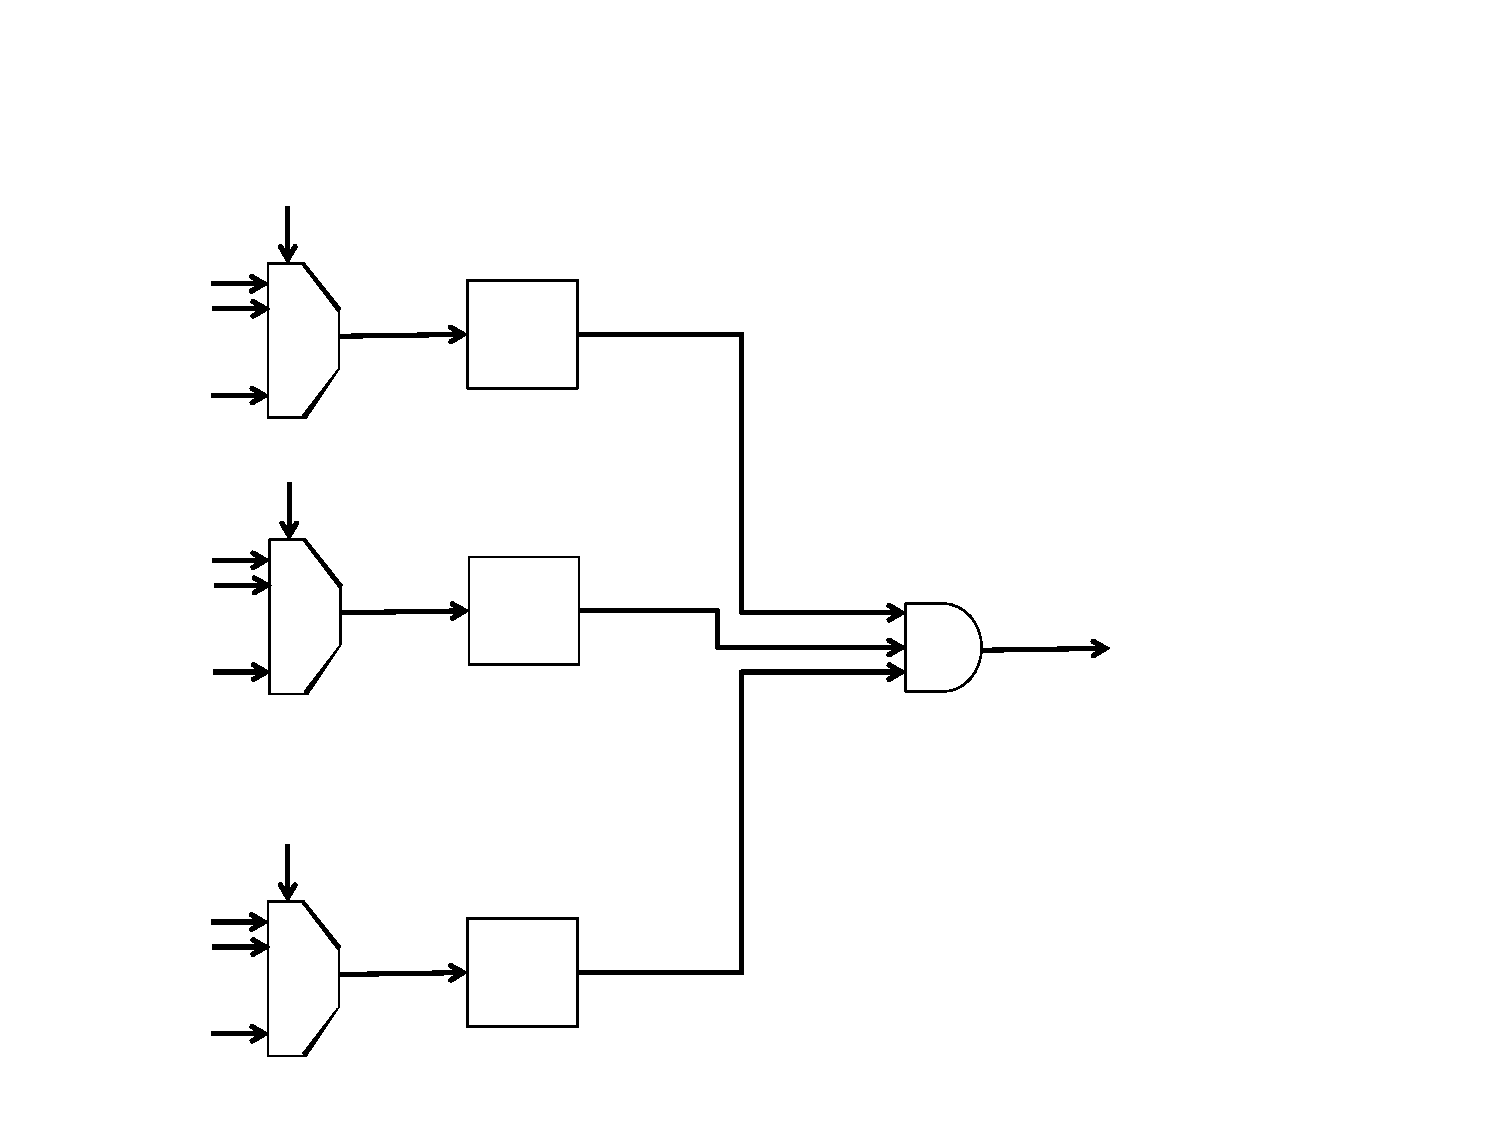
\includegraphics[scale=0.5]{atpg_circuit}
%\begin{overpic}[scale=0.5,unit=1mm,grid]{atpg_circuit}
\begin{overpic}[scale=0.5,unit=1mm]{atpg_circuit}
    \put(11,74){$\bar{s_1}$}
    \put(1,67){$p_1$}
    \put(1,64){$p_2$}
    \put(2, 62){$.$}
    \put(2, 61){$.$}
    \put(2, 60){$.$}
    \put(1,57){$p_m$}
    \put(30,61){$C^{f}_1$}
    
    \put(11,50){$\bar{s_2}$}
    \put(1,43){$p_1$}
    \put(1,40){$p_2$}
    \put(2, 38){$.$}
    \put(2, 37){$.$}
    \put(2, 36){$.$}
    \put(1,33){$p_m$}
    \put(30,38){$C^{f}_2$}
    
    \put(25, 30){$.$}
    \put(25, 26){$.$}
    \put(25, 22){$.$}
    \put(25, 18){$.$}
    
    \put(11,20){$\bar{s_k}$}
    \put(1,13){$p_1$}
    \put(1,10){$p_2$}
    \put(2, 8){$.$}
    \put(2, 7){$.$}
    \put(2, 6){$.$}
    \put(1,3){$p_m$}
    \put(30,7){$C^{f}_k$}
    
    \put(82,34.5){$T^m_k$}
\end{overpic}
\caption{A representation of the circuit used to implement \textbf{testSet}($\Phi$, $G$, $m$), where $k = |G|$.  For each fault $i$ in $G$, there is a corresponding sub-circuit $C^f_i$. The input lines $p_1,...,p_m$ correspond to the $m$ test patterns. A multiplexer with selector variables $\bar{s_i}$ is used to select which test pattern will be sent to $C^f_i$. There is a set of inputs $p_1,..,p_m$ and $\bar{s_1},..,\bar{s_k}$ such that $T^m_k = 1$, if and only if there is a test set of size $m$ that detects all faults in $G$.}
\label{fig:circuit}
\end{figure}


\begin{figure}[t]
\centering
\begin{overpic}[scale=0.5,unit=1mm]{subcircuit}
\put(1,9){$p_k$}
\put(41,9){$C^f_i$}
\put(17.5,14){$\Phi$}
\put(17,3.5){$\Phi^f_{i}$}
\end{overpic}
\caption{A representation of one sub-circuit $C^f_i$ from Figure~\ref{fig:circuit}, that asserts that fault $i$ of circuit $\Phi$ is detected. The output of the original circuit $\Phi$ is compared to the output of the faulty circuit $\Phi^f_i$ using an XOR.}
\label{fig:subcircuit}
\end{figure}

\subsection{Incremental SAT Solving}
The \textbf{testSet} function is called in each iteration of Algorithm~\ref{algo:atpg1}, after either a new fault has been added to $G$, or the value of $m$ has been increased. It is obvious that the CNF formula (described in Section~\ref{sec:testsetimpl}) generated during a call to \textbf{testSet} will be very similar to the CNF formula generated in the previous iteration. Therefore, it may be beneficial to use an incremental SAT solver that can exploit this relationship, instead of solving each SAT instance independently.\\

In this section we specify which clauses must be added and removed from the CNF formula, when either $G$ is augmented or $m$ is increased. In our implementation, we use the incremental interface of Minisat to add clauses, as well as Minisat's support for solving under assumptions, to remove clauses. We hope that the clauses learned by Minisat in previous calls to the solve routine will improve the performance of subsequent calls.\\

\subsubsection{Adding a Fault}
When a fault $i$ is added to $G$, we must add a new sub-circuit $C^f_i$ to the formula shown in Figure~\ref{fig:circuit}. We must also add a new multiplexer that feeds into $C^f_i$. It is not hard to see that we only need to \textit{add} clauses to the current formula, and we do not have to remove any clauses in this case. 
 
\subsubsection{Increasing the Test Set Size}           
When the number of test patterns is incremented by $1$, we must add a new set of input variables $p_{m+1}$ to the formula. Each existing multiplexer must be augmented with $p_{m+1}$, which requires adding a new selector variable to the multiplexer as well. The only clauses that need to be removed are the ones saying that at least one selector variable must be True. Now, each such clause must be replaced with a longer version of it, where the new selector variable has been added to the disjunction.  That is, $(s_1\vee,...,\vee s_m)$ is removed, and $(s_1\vee,...,\vee s_m \vee s_{m+1})$ is added instead.   

\section{Related Work}

The \MCCC problem was proven to be NP-hard by Krishnamurthy and Akers in 1984~\cite{Krishnamurthy:1984:CES:1907650.1907919}.\\

Almost all work on ATPG assumes that it is computationally infeasible to find an MCCC. Most existing approaches consider the faults one at a time, and  use a SAT solver to find a test pattern for each fault. \\

Reddy et al. consider structural (rather than SAT-based) approaches for ATPG, and propose various heuristics for compact test set generation~\cite{pomeranz93,10.1109/TEST.2013.6651914}. Some work on SAT-based ATPG proposes to exploit the internal data structures of the SAT solver~\cite{5359362}. Recently, there has been increased interest in SAT-based methods to produce compact test sets~\cite{6628311,DBLP:journals/it/EggersglussD14,6847807,10.1109/VLSID.2014.17}. There is also work that attempts to throw out redundant test patterns, after a set of test patterns that covers all faults has been determined. Given a set of test patterns and the list of faults that each pattern detects, a minimum set covering problem can be set up to find the minimum size subset of the patterns that still detects all faults~\cite{conf/glvlsi/FloresNS99}. Note that this will not necessarily find an \MCCC, since the size of the resulting minimized test set depends on the initial set of test patterns.\\ \\

The only existing work on calculating an optimal \MCCC is by Marques Silva\footnote{Marques Silva calls the \MCCC problem the \textit{minimum test set} problem.}, who proposed an encoding of the \MCCC problem to an Integer Linear Programming (ILP) problem~\cite{DBLP:conf/aspdac/Silva98}. However, the ILP model is of size $O(n^3)$ where $n$ is the size of the original circuit $\Phi$, and the number of faults $|\F|$. Marques Silva does not report any experimental results  concerning this translation to ILP. For large circuits with tens or hundreds of millions of gates and faults, the size of this ILP model, not to mention the additional memory required to solve it using Branch and Cut, is expected to be prohibitive. \\


As an example of a SAT-based approach that performs dynamic compaction, we describe the algorithm from~\cite{10.1109/VLSID.2014.17}. The faults are first ordered according to a topological criteria. At each iteration of the algorithm, a group of faults is built up in a greedy manner. The group of faults must satisfy the criterion that a single test pattern can detect all faults in the group. This is done by checking whether or not the next fault in the list can be added to the current group while maintaining the criterion. The iteration ends after a certain number of faults have been rejected from the current group\footnote{Rejected faults are placed back on the list, to be retried in the next iteration.}.  At the end of the iteration, a test pattern that detects all faults in the group is added to the final test set. This test pattern is then used for fault simulation, to remove other detected faults from the fault list. The next iteration begins with a new fault group, containing the next undetected fault in the list. The intuition for this approach is that it finds test patterns that can detect many faults, by finding groups of faults that can be detected using a single test pattern. \\


\section{Experimental Results}
TIGUAN is a recent SAT-based ATPG tool that performs dynamic compaction~\cite{10.1109/VLSID.2014.17}. It supports a richer fault model, but can also handle stuck-at faults. Although TIGUAN is not publicly available,~\cite{10.1109/VLSID.2014.17} reports the size of the test sets generated for all stuck-at faults\footnote{Alexander Czutro, private communication} in a subset of ISCAS'85 and ISCAS'89 circuits.

Experiments were performed on ISCAS85, ISCAS89, and ITC99 circuits~\cite{iscasTGPRO}.

\section{Alternative Approach Using Min-MUS}
Let $F = F_0 \cup F_1$ be the set of detectable faults of circuit $\Phi$, where $F_0$ and $F_1$ are the stuck-at-0 and stuck-at-1 faults respectively. Suppose we have already found a test set $S = \{p_1,...,p_k \}$ that is complete for $F$ (here, $S$ can be of arbitrary size). We define the following propositional formula $\Theta_S$\footnote{This formula is similar to the one defined by Fujita and Mishchenko~\cite{fujita14}, except here we constrain the number of simultaneous faults to be 1.}:

\begin{displaymath}
\Theta_S = \bigwedge_{p_i \in S}\left[(C_i(p_i)=o_i) \bigwedge_{j\in F_1}(\neg f_j \vee \ell^i_j) \bigwedge_{j \in F_0}(\neg f_j \vee \neg \ell^i_j) \right] \wedge \left[ \Sigma_{j \in F}f_j = 1 \right]
\end{displaymath} 

where $C_i(p_i)$ is the formula consisting of a copy of circuit $\Phi$ with its inputs set to $p_i$, and $o_i = \Phi(p_i)$ is a constant equal to the value of the output lines in the correct circuit $\Phi$ on input $p_i$. There is a fault variable $f_j$ for each fault $j\in F$, and exactly one of these variables must be assigned to True. Finally, $\ell^i_j$ is the variable in $C_i(p_i)$ corresponding to the line affected by fault $j\in F$.\\


If $\Theta_S$ is satisfiable, then there exists a fault $j \in F$ such that the output of the faulty circuit is the same as the output of $\Phi$ for all $p_i \in S$. Therefore, $S$ is not a complete test set.

\begin{proposition}
$\Theta_S$ is unsatisfiable if and only if $S$ is a complete test set.
\end{proposition}


\begin{proposition}
If $\Theta_S$ is unsatisfiable, then a minimal unsatisfiable core of $\Theta_S$ corresponds to a minimal complete test set.
\end{proposition}

\begin{proposition}
\label{prop:minmus}
There exists a complete test set $S$ such that an unsatisfiable core of $\Theta_S$ of minimum size corresponds to a \MCCC.
\end{proposition}

Proposition~\ref{prop:minmus} suggests an alternative algorithm for finding a \MCCC. We propose to find a complete test set $S$ using existing heuristic methods, e.g.~\cite{czutro14}. Given $S$, we build $\Theta_S$ and find a minimal or min-size core using existing methods such as~\cite{belov12,ignatiev13}.         
\bibliographystyle{plain}
\bibliography{atpg}
\end{document}
